\begin{frame}
	\begin{center}
		\Huge Kampf
	\end{center}
\end{frame}

\begin{frame}
	\frametitle{Das Kampfkonzept}
		\begin{itemize}
		\item Klick auf den Lehrer $\rightarrow$ Kampf startet
		\item Spieler greift an $\rightarrow$ Lehrer verteidigt
		\item Lehrer greift an $\rightarrow$ Spieler verteidigt 
		\item Schaden entspricht der Differenz der Item-Stärken
		\item Lebenspunkte um Schaden reduziert
		\item bei 0 oder weniger Lebenspunkten: verloren
	\end{itemize}
\end{frame}


\begin{frame}
	\frametitle{Funktion: getItems}
	\begin{figure}
		\centering
		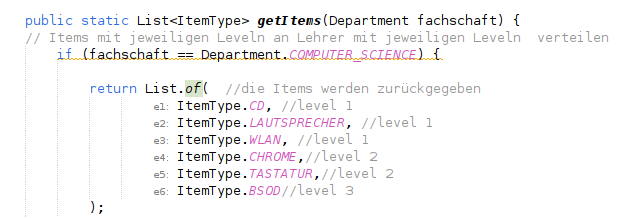
\includegraphics[width=.8\textwidth]{bilder/GetItems.png}
		\caption{Ausschnitt der Funktion getItems (Bildschirmfoto des Projektes)}
		\label{fig:agi}
	\end{figure}
\end{frame}

\begin{frame}
	\frametitle{Lehrer-Funktion}
		\begin{figure}
		\centering
		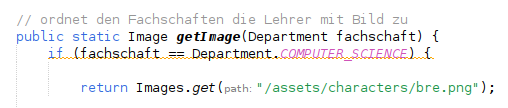
\includegraphics[width=.6\textwidth]{bilder/Lehrer-Funktion.png}
		\caption{Ausschnitt der Funktion getItems (Bildschirmfoto des Projektes)}
		\label{fig:alf}
	\end{figure}
\end{frame

\begin{frame}
	Erst erklären warum Idee I nicht funktioniert.\\
	Dann Idee zwei erklären.\\
	\begin{itemize}
		\item Update Funktion noch einmal einführen
		\item warum sie uns hilft
		\item verschiedene updates erklären
		\item noch draw Funktion ansprechen
	\end{itemize}
\end{frame}
